\documentclass[dvipdfmx, dvipsnames]{beamer}
\usetheme[secheader]{Boadilla}
% \usepackage{beamerthemesplit} // Activate for custom appearanced
%\setbeamertemplate{caption}[numbered]
\usefonttheme[onlymath]{serif} %数式をゴシックにしない
%\setbeamertemplate{blocks}[rounded] % Blockの影を消す
\useinnertheme{circles} % 箇条書きをシンプルに
\setbeamertemplate{navigation symbols}{} % ナビゲーションシンボルを消す
\setbeamertemplate{footline}[frame number] % フッターはスライド番号のみ
\setbeamercolor{page number in head/foot}{fg=black}
% \usepackage{beamerthemesplit} // Activate for custom appearance
%\setlength{\parindent}{1em}  %段落字下げ
\renewcommand{\figurename}{Fig}
\renewcommand{\tablename}{Tab}
\usepackage[caption=false]{subfig}
%\usepackage{blindtext}
\usepackage{tikz}
\usetikzlibrary{decorations.pathreplacing,calligraphy}
\usetikzlibrary{angles,quotes} % for pic
%\setbeamerfont{itemize/enumerate subbody}{size=\normalsize} %subitem を同じ大きさに
%
%\setbeamertemplate{itemize subitem}{\normalsize\raise1.25pt\hbox{\donotcoloroutermaths$\blacktriangleright$}}  %to set the symbol size
\usetikzlibrary{shapes,positioning}
\usepackage{xcolor}

\def\mathunderline#1#2{\color{#1}\underline{{\color{black}#2}}\color{black}}

\setbeamercolor{block title}{bg=gray!10} %block title の背景
\setbeamercolor{block body}{bg=white} %block の中身

%def symbol
\newcommand{\normal}{\mathcal{N}}
\newcommand{\exponential}{\mathcal{E}}
\newcommand{\truncnorm}{\mathcal{TN}}
\newcommand{\gam}{\mathcal{G}}
\newcommand{\C}{C}
\newcommand{\one}{1\!\!1}

%list を black-right-triangle にするコマンド
\newcommand{\triangleitem}{
\setbeamertemplate{itemize item}{\color{RedOrange}$\blacktriangleright$}
\setbeamertemplate{itemize subitem}{\color{RedOrange}$\blacktriangleright$}
}

\title{テンソル同時分解の拡張による\\オミクスデータの統合}
\date{2024年5月25日}
\author {阿部興\footnote{東京医科歯科大学難治疾患研究所} ・島村徹平\footnote{名古屋大学医学系研究科・東京医科歯科大学難治疾患研究所}}

\begin{document}
\frame{
\titlepage
}

\renewcommand*{\thefootnote}{\fnsymbol{footnote}}
\setcounter{footnote}{0} 

\section{背景}
\frame{
\frametitle{動機:分析対象}
\begin{figure}
 \begin{tikzpicture}
\node[draw, rounded corners, fill=gray!10](dna) at (0,0){
\includegraphics[width=.05\textwidth]{img/dna.png}DNA};
\node[draw, rounded corners, fill=gray!10, right = of dna, xshift = +15pt](rna){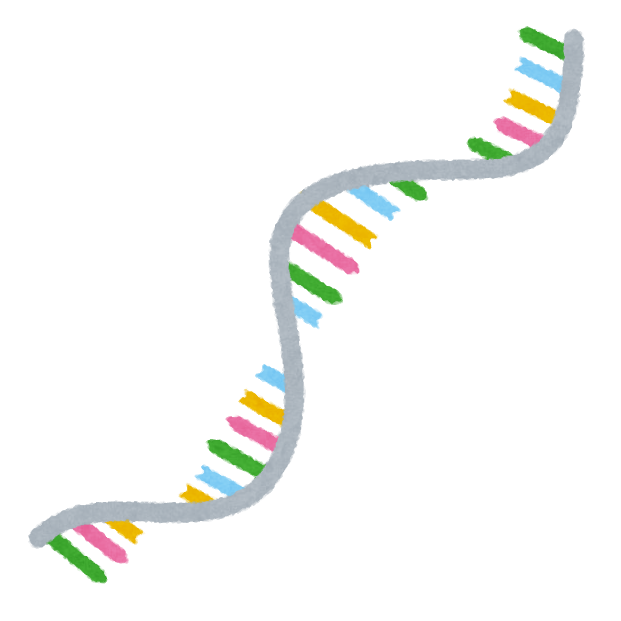
\includegraphics[width=.05\textwidth]{img/body_rna.png}RNA};
\node[draw, rounded corners, fill=gray!10, right = of rna, xshift = +15pt](protein){
\includegraphics[width=.05\textwidth]{img/kagaku_bunshi.png}protein};
\node[draw, rounded corners, fill=gray!10, right = of protein](phenotype) {
\includegraphics[width=.05\textwidth]{img/nut_renzumame.png}phenotype};
%path
\path[draw, ->, darkgray](dna)--(rna) node[midway, below, yshift = -2pt]{転写};
\path[draw, ->,darkgray](rna)--(protein) node[midway, below, yshift = -2pt]{翻訳};
\path[draw, dashed, ->, darkgray](protein)--(phenotype);
%omics
\node[below= of dna](genomics){genomics};
\node[below= of rna](transcriptomics){transcriptomics};
\node[below= of protein](proteomics){proteomics};

\node[above= of dna, yshift=-5ex]{\textcolor{darkgray}{モダリティ}};

\path[draw, RoyalBlue](dna)--(genomics);
\path[draw, RedOrange](rna)--(transcriptomics);
\path[draw, RedOrange](proteomics)--(protein);

\path[draw, RedOrange, dashed](genomics.north west)--(proteomics.north east);
\path[draw, RedOrange, dashed](genomics.south west)--(proteomics.south east);
\path[draw, RedOrange, dashed](genomics.north west)--(genomics.south west);
\path[draw, RedOrange, dashed](proteomics.north east)--(proteomics.east)node[right](omics){-omics};
\end{tikzpicture}
\caption{遺伝子発現の情報の流れ}
\end{figure}

モダリティ(計測対象)が違っても普遍的な現象があるはず

\triangleitem
\begin{itemize}
\item オミクス(omics)データを統合して分析したい
\end{itemize}
}
\frame{
\frametitle{データ統合}
\begin{figure}
 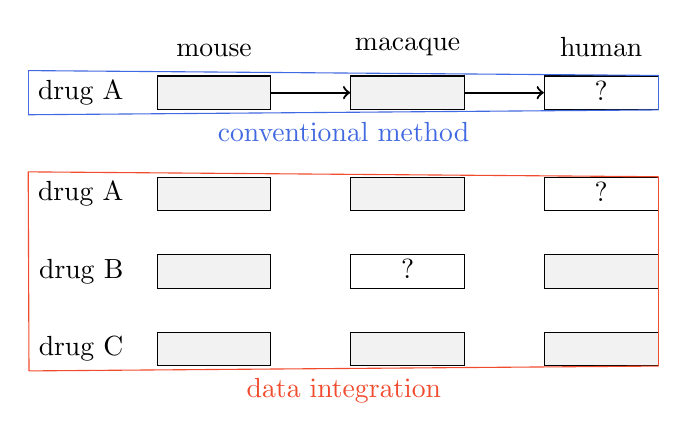
\begin{tikzpicture}
\node[draw, fill=gray!10, text height=1.25ex, text width=8.0ex](mouse) at (0,0){   };
\node[draw, fill=gray!10, right = of mouse, text height=1.25ex, text width=8.0ex](lemur){};
\node[draw,  right = of lemur, text height=1.25ex, text width=8.0ex, align=center](human){?};

\node[above = of mouse, yshift = -25pt] (labmouse){mouse};
\node[above = of lemur, yshift = -25pt](lablemur){macaque};
\node[above = of human, yshift = -25pt](labhuman){human};

\path[draw,->, thick](mouse)--(lemur);
\path[draw,->, thick](lemur)--(human);

\node[left = of mouse, xshift = 20pt] (labA){drug A};

\node[draw, fill=gray!10, text height=1.25ex, text width=8.0ex, below=of mouse, yshift = 1ex](mouse2){};
\node[draw, fill=gray!10, right = of mouse2, text height=1.25ex, text width=8.0ex](lemur2){};
\node[draw,  right = of lemur2, text height=1.25ex, text width=8.0ex, align=center](human2){?};

\node[draw, fill=gray!10, text height=1.25ex, text width=8.0ex, below=of mouse2, yshift = 3ex](mouse3){};
\node[draw, right = of mouse3, text height=1.25ex, text width=8.0ex, align=center](lemur3){?};
\node[draw, fill=gray!10, right = of lemur3, text height=1.25ex, text width=8.0ex, align=center](human3){};

\node[draw,  fill=gray!10, text height=1.25ex, text width=8.0ex, below=of mouse3, yshift = 3ex](mouse4){};
\node[draw, fill=gray!10, right = of mouse4, text height=1.25ex, text width=8.0ex](lemur4){};
\node[draw,  fill=gray!10, right = of lemur4, text height=1.25ex, text width=8.0ex, align=center](human4){};

\node[left = of mouse2, xshift = 20pt] (labA2){drug A};
\node[left = of mouse3, xshift = 20pt] (labB){drug B};
\node[left = of mouse4, xshift = 20pt] (labC){drug C};

\def \intcol {RedOrange};
\path[draw,  \intcol ](labA2.north west)--(human2.north east);
\path[draw,  \intcol ](labA2.north west)--(labC.south west);
\path[draw,  \intcol ](human2.north east)--(human4.south east);
\path[draw,  \intcol ](labC.south west)--(human4.south east)node[midway, below](int){data integration};

%
\def \convcol {RoyalBlue};
\path[draw, \convcol](labA.north west)--(human.north east);
\path[draw, \convcol](labA.north west)--(labA.south west);
\path[draw, \convcol](human.north east)--(human.south east);
\path[draw, \convcol](labA.south west)--(human.south east)node[midway, below](single){conventional method};
\end{tikzpicture}
%\caption{データ統合により情報を補完しあう}
\end{figure}

\begin{description}
\item[積極的動機] データを補い合い普遍的な特徴を抽出
\item[消極的動機] 対応のあるサンプルなので非独立
\end{description}

\triangleitem
\begin{itemize}
\item semi-paired なデータが多い
\item モダリティごとに分布が変わる
\end{itemize}
}
\frame{
\frametitle{動機:分析手法}
\begin{figure}
\begin{tabular}{c|c}
\footnotesize multi-dimensional array & \footnotesize tidy format\footnotemark[1]\\
\hline
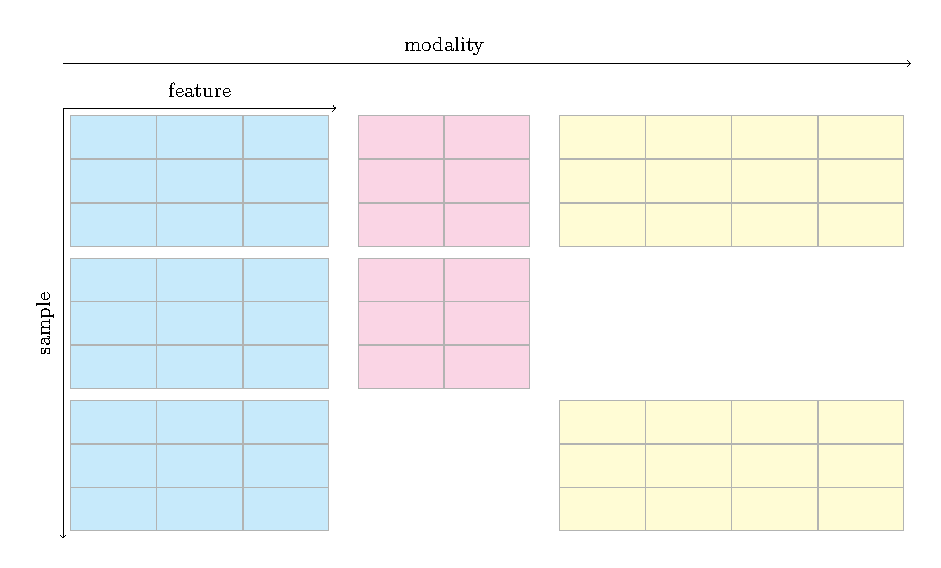
\includegraphics[height=0.4\textheight]{img/mmdata} &
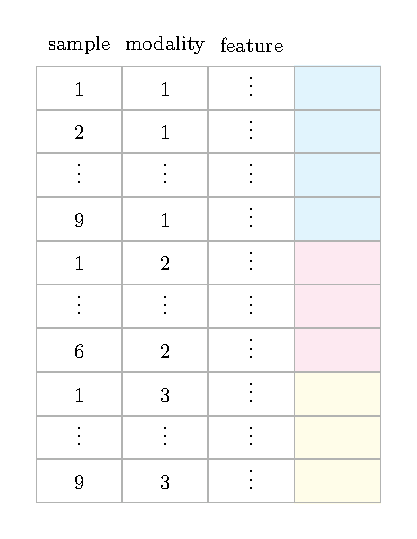
\includegraphics[height=0.4\textheight]{img/mm_tidy} \\
\end{tabular}
\caption{semi-paired なマルチオミクスデータ. 左右で持つ情報は同じ.}
\end{figure}

tidy format は欠測や反復測定の扱いに優れる

\footnotetext[1]{Wickham H. (2019).  {\em Advanced R, second edition}. Chapman and Hall/CRC.} 
}
\frame{
\frametitle{動機:分析手法}
\begin{figure}
\begin{tabular}{c|c}
\footnotesize multi-dimensional array & \footnotesize tidy format\footnotemark[1]\\
\hline
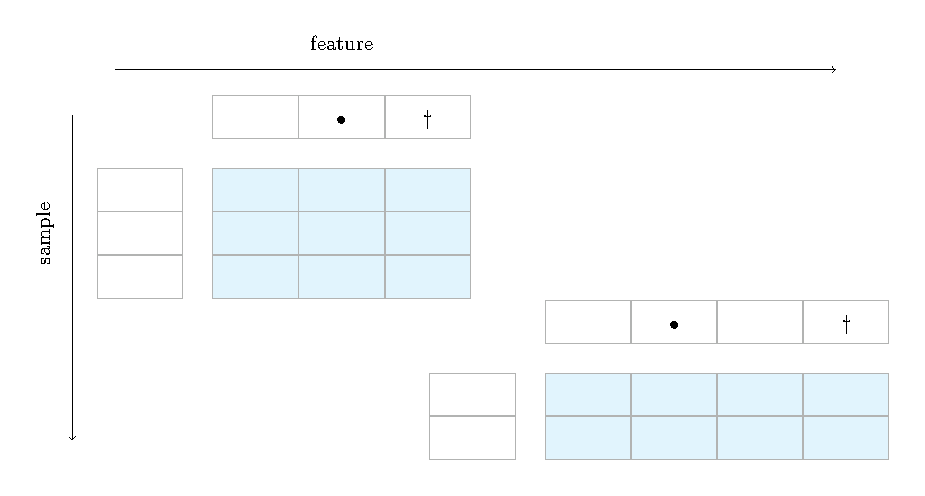
\includegraphics[height=0.4\textheight]{img/anndata} & 
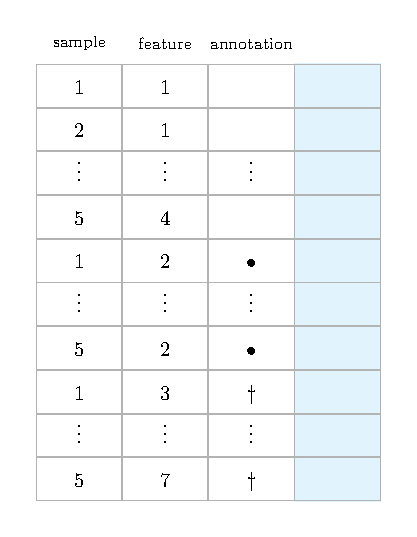
\includegraphics[height=0.4\textheight]{img/ann_tidy}
\end{tabular}
\caption{アノテーションつきのオミクスデータ. 左右で持つ情報は同じ.}
\end{figure}

%tidy format: multi-dimensional array と持つ情報は同じだが欠測や繰り返し測定の扱いに優れる
\setbeamertemplate{itemize item}{\color{RedOrange}$\blacktriangleright$}
\begin{itemize}
\item tidy format の利便性を生かしたまま行列分解ができないか?
\end{itemize}

\footnotetext[1]{Wickham H. (2019).  {\em Advanced R, second edition}. Chapman and Hall/CRC.} 
}
\frame{
\frametitle{提案モデル(準備)}
\begin{columns}
\begin{column}{0.4\textwidth}
\begin{figure}
\centering
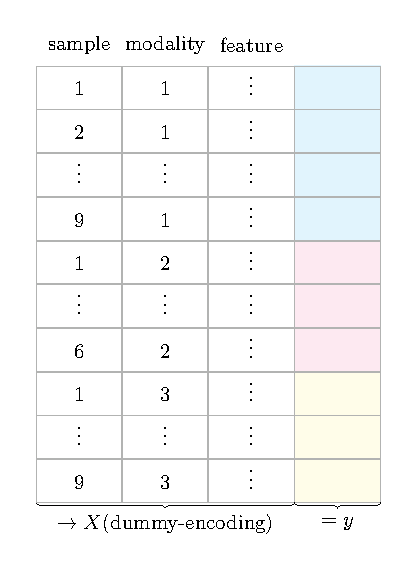
\includegraphics[width=\textwidth]{tikzfig/tidy_concept.pdf} 
\end{figure}
\end{column}
\begin{column}{0.6\textwidth}
観測モデル:正規分布\footnotemark[1]
\begin{align*}
y_n \mid V, \lambda & \sim \normal\left(y_n \mid \sum_{l=1}^L \prod_{d=1}^D v_{dl}^{x_{nd}}, \lambda^{-1}\right)
\end{align*}

事前分布:区間 $(0,\infty)$ に切断された正規分布, ガンマ分布
\begin{align*}
v_{dl} & \sim \truncnorm_{(0,\infty)}(v_{dl} | 0,\tau^{-1}) \quad\\
\lambda & \sim \gam(\lambda | a,b) %(shape $=a$, rate $=b$)}%\nonumber
\end{align*}
\end{column}
\end{columns}
\footnotetext[1]{cf. Abe \& Shimamura (2023). UNMF: A unified non-negative matrix factorization for multi-dimensional omics data. \textit{Briefings in Bioinformatics.}  ではポアソン分布を仮定}
}

\frame{
\frametitle{内積としての解釈}
\begin{align*}
y_{n}  \approx\sum_{l=1}^L \prod_{d=1}^D v_{dl}^{x_{nd}} &= v_{11}^{x_{n1}} v_{21}^{x_{n2}}\cdots  v_{D1}^{x_{nD}}+ \cdots + v_{1L}^{x_{n1}} v_{2L}^{x_{n2}}\cdots  v_{DL}^{x_{nD}}\\
&=
 \underbrace{
 \color{RedOrange}
\begin{pmatrix}
v_{d1}^{x_{nd}} &  \ldots  & v_{dL}^{x_{nd}}
 \end{pmatrix} 
 \color{RoyalBlue}
 \begin{pmatrix}
\prod _{d' \neq d}v_{d'1}^{x_{nd'}}\\
 \vdots \\
 \prod _{d' \neq d}v_{d'L}^{x_{nd'}}
 \end{pmatrix}
 }_{\mbox{inner product}}
\end{align*}

\begin{figure}
\begin{tabular}{ccc}
inner product of \Huge $($
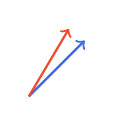
\begin{tikzpicture}
\draw[thick,->,color=RoyalBlue] (0,0)--(0.71,0.71); 
  \draw[thick,->,color=RedOrange] (0,0)--(0.51,0.86);
\end{tikzpicture}
$)$
&
\Large $>$
&
inner product of \Huge $($
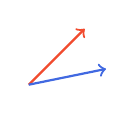
\begin{tikzpicture}
 \draw[thick,->,color=RedOrange] (0,0)--(0.71,0.71);
  \draw[thick,->,color=RoyalBlue] (0,0)--(0.98,0.2);
\end{tikzpicture}
$)$
\end{tabular}
\caption{$y_n$の値が大きいとき$V$の$X$ で指定される成分どうしの値が似る}
\end{figure}
}
\frame{
\frametitle{アンサンブルとしての解釈}
\begin{align*}
y_{n}  \approx\ &\sum_{l=1}^L\prod_{d=1}^D v_{dl}^{x_{nd}} \\
&=\frac{1}{L}\sum_{l=1}^L \underbrace{ L\exp\left( \sum_{d=1}^D x_{nd}  \cdot \log v_{dl}\right) }_{\mbox{log-linear model}}
%&= \frac{1}{L}\sum_{l=1}^L L f_{nl} \quad \mbox{\structure{(mean of the log-linear predictor)}}
\end{align*}
\begin{figure}
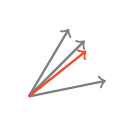
\begin{tikzpicture}
\draw[thick,->,color=gray] (0,0)--(0.71,0.71); 
\draw[thick,->,color=gray] (0,0)--(0.51,0.86);
\draw[thick,->,color=gray](0,0)--(0.98,0.2);
\draw[thick,->,color=RedOrange](0,0)--(0.73,0.58);
\end{tikzpicture}
\caption{複数の対数線形モデルの平均と捉えられる}
\end{figure}
}

%\frame{
%\frametitle{事前分布:非負制約}
%\begin{align*}
%v_{dl} & \sim \truncnorm(v_{dl} | 0,\tau^{-1})  \quad \mbox{\footnotesize 切断正規分布}\\
%& \propto \normal(v_{dl} | 0,\tau^{-1})\one_{(0,\infty)}(v_{dl})
%\end{align*}
%ここで, $\one_{A}(x)$ は指示関数($x \in A$ のとき1,さもなくば0).
%
%\vspace{\baselineskip}
%
%\structure{Note:} 原理的には, 非負制約の有無は変数ごとに選ぶこともできるが, 今回は煩雑さを避けるためすべて非負とした.
%}
\frame{
\frametitle{中間変数:分布を変える}
\begin{itemize}
\item $y_n$ が実数(連続値):恒等変換
$$
A(z_n)=z_n.
$$
\item 
$y_n$ が非負:非負化
$$
A(z_n)=\begin{cases}z_n, &z_n>0\\0 &z_n\leq 0\end{cases}
$$
\item
$y_n$ が2値(0 or 1):2値化
$$
A(z_n)=\one_{(0,\infty)}(z_n)  \quad \mbox{\footnotesize \structure{(indicator function)}}
$$
\item
$y_n$ が非負の整数:離散化
$$
A(z_n)=\begin{cases}\lceil z_n\rceil, & z_n>0  \quad \mbox{\footnotesize \structure{(ceiling function)}}
\\0 &z_n \leq 0\end{cases}
$$
\end{itemize}
}
\frame{
\frametitle{切断, 非負化, 離散化}
\begin{figure}
\centering
\begin{tabular}{c|cc}
\subfloat[切断]{ 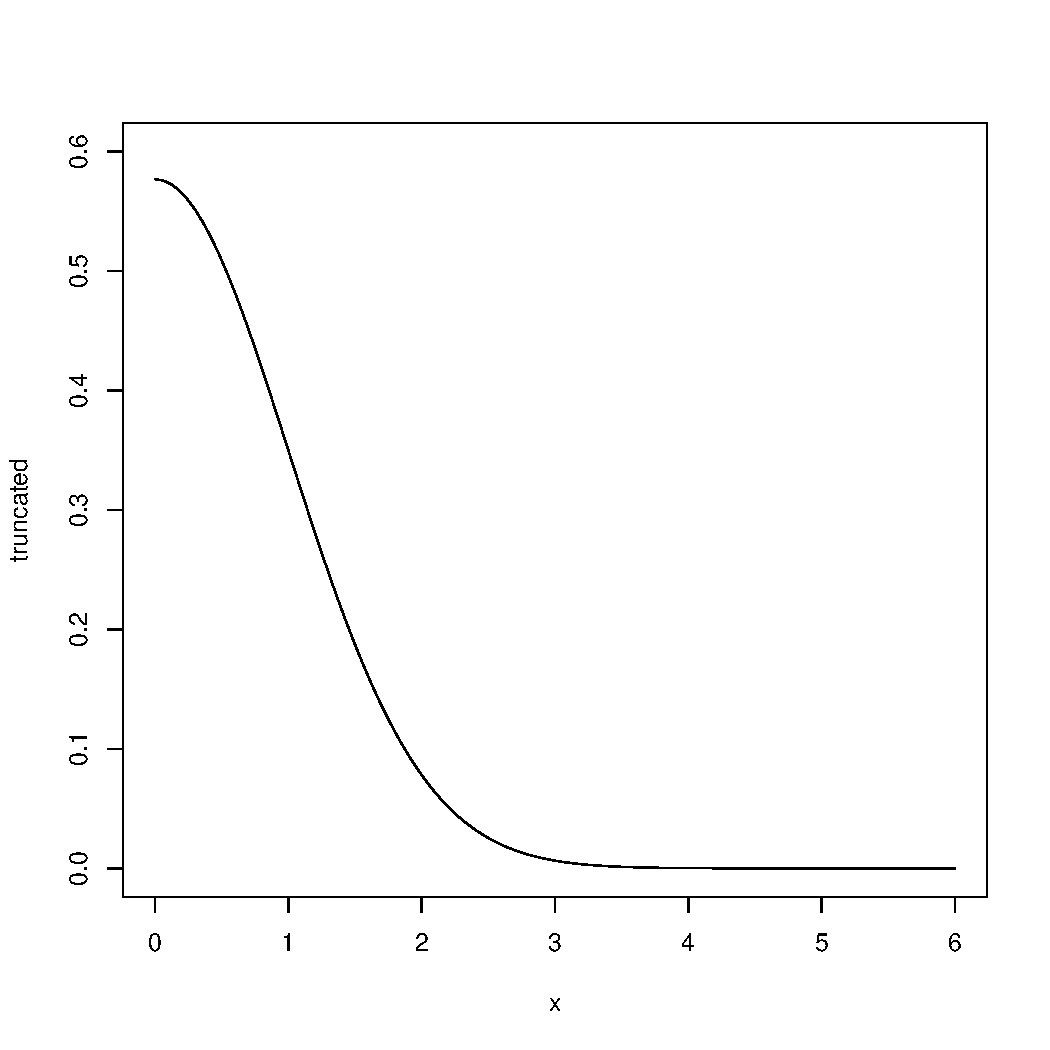
\includegraphics[width=0.3\textwidth]{img/norm_truncated}}&
\subfloat[非負化]{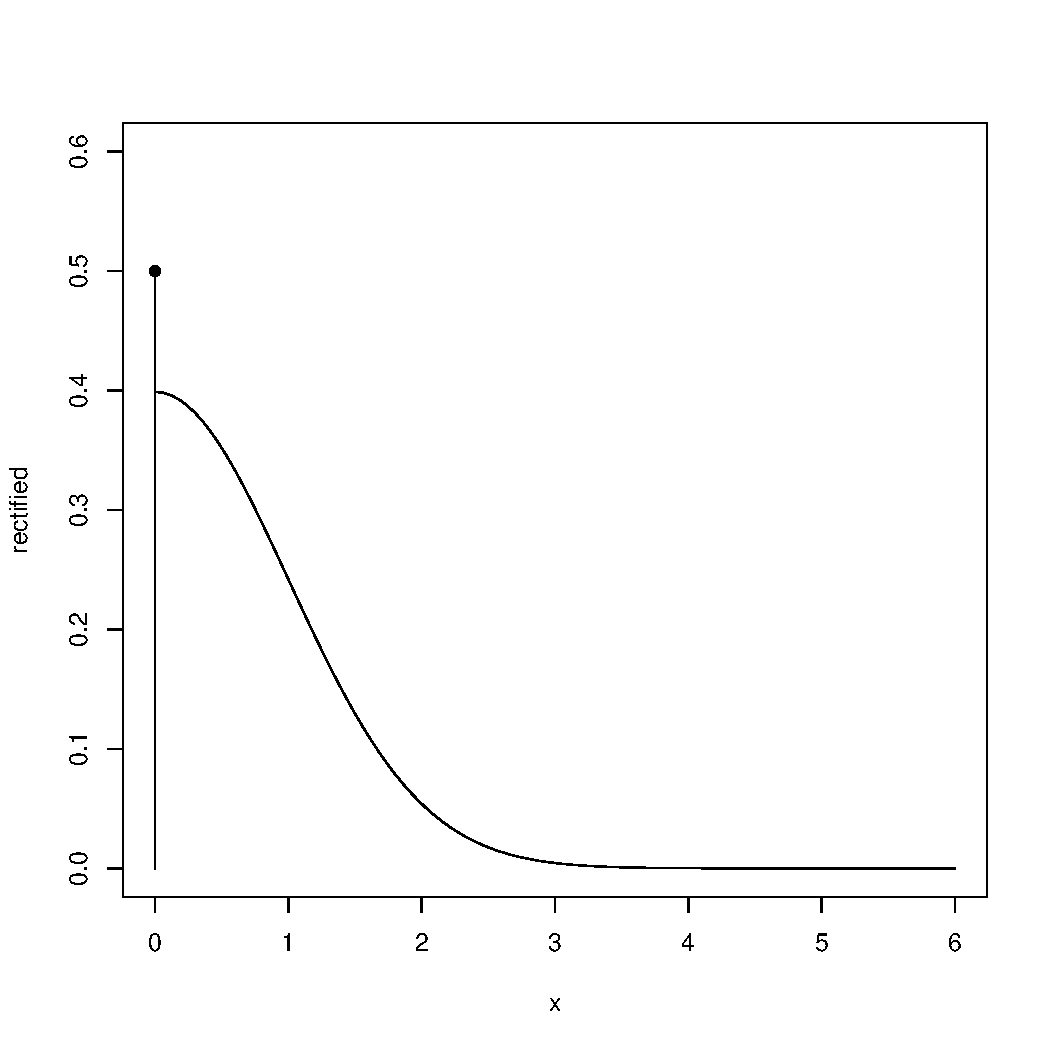
\includegraphics[width=0.3\textwidth]{img/norm_rectified}}&
\subfloat[離散化]{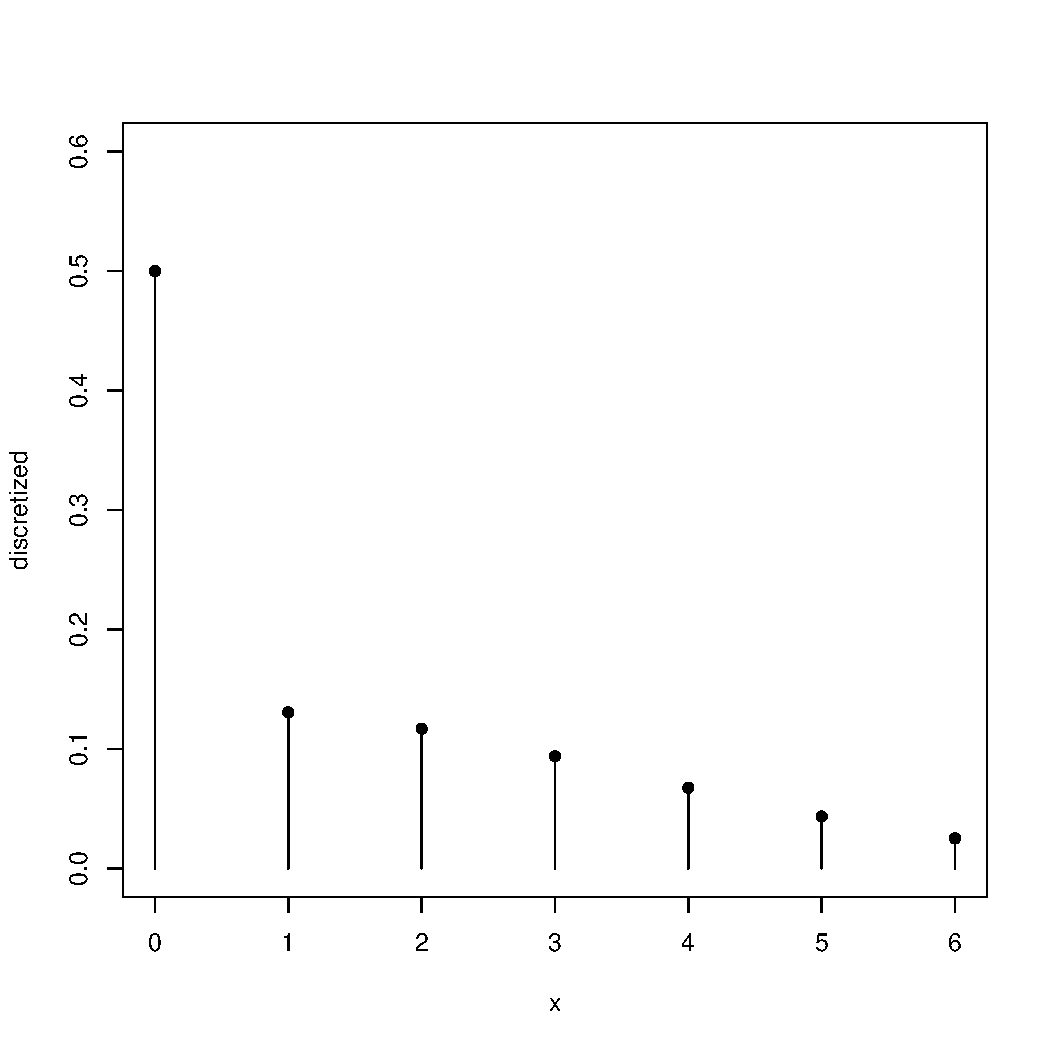
\includegraphics[width=0.3\textwidth]{img/norm_discretized}}
\end{tabular}
\caption{a: 潜在変数の事前分布. b, c: 観測されるデータのモデル. 観測されるデータのモデルは0の一点で確率を持つ(cf. zero-inflated モデル)}
\end{figure}

%\vspace{\baselineskip}

\structure{Note:} モデルの密度が0になることは対数尤度に$-\infty$の罰則をつけることと同じであるため, 分布の台が特に重要と考えた.
}
\frame{
\frametitle{提案モデル}

\begin{equation*}
y_{n} = A_{m(n)}(z_{n}), \quad z_{n} \sim \mathcal{N}\left(\sum_{l=1}^L \prod_{d=1}^Dv_{dl}^{x_{nd}}, \lambda^{-1}\right)% \label{eq_mod2}    
\end{equation*}
ここで $m(n)$ は $n$ をモダリティを区別する添字に写す関数. 

\begin{block}{分析者が設定する要素(チューニングパラメータ)}
\begin{itemize}
\item[] 潜在変数$V$の次元$L$
\item[] 中間的関数$A(x)$
\item[] 計画行列$X$
\item[] 事前分布のパラメータ $\tau$, $a$, $b$
\end{itemize}
\end{block}
}
\frame{
\frametitle{対数尤度}
\begin{align*}
 \ell(v_{dl}) &=\sum_{n=1}^{N} \log p(z|V, X) = \sum_{n=1}^{N}\left(-\frac{\lambda}{2}\left\{ z_n -\sum_{l=1}^L\prod_{d=1}^D v_{dl}^{x_{nd}} \right\}^2\right)+ \C\\
&= -\frac{h_{dl}}{2}\left(v_{dl}^2-2v_{dl}\frac{\eta_{dl}}{h_{dl}}\right) +C,
\end{align*}
ここで,
\begin{align*}
\eta_{dl} &= \sum_n x_{nd} \prod_{d' \neq d} v_{dl}^{x_{nd}}\left( z_{n} - \sum_{l'\neq l} \prod_{d' \neq d} v_{dl}^{x_{nd}} \right), \quad \mbox{\footnotesize 1次の項} \\ %\label{eq_eta}\\
h_{dl} &= \sum_n \lambda x_{nd} \prod_{d' \neq d} v_{dl}^{2x_{nd}}, \quad \mbox{\footnotesize 2次の項}% \label{eq_h}
\end{align*}
$v_{dl}$ に依存しない定数をまとめて $C$ とした.
}
\frame{
\frametitle{変分EMアルゴリズム(一般論)}

\begin{itemize}
\item[] データ: $\mathcal{D}=(\mathcal{D}_1,\mathcal{D}_2,\ldots,\mathcal{D}_n)$ 
\item[] $\mathcal{D}$ 全体に影響する \structure{global} な潜在変数: $V$
\item[] $\mathcal{D}_n$ に影響する \structure{local} な潜在変数: $z_n$ ($z=(z_1,\ldots,z_N)'$)
\end{itemize}

\begin{align*}
D_{KL}(q\|p) &=\int q(z) \log \frac{q(z)}{p(z_n|\mathcal{D},w)} dz\\
&= E_q [ \log q(z)] - E_q[\log p(z_n|\mathcal{D},w)]
\end{align*}
$q(z) \propto  \exp( E_q[\log p(z_n|\mathcal{D},w)])$ のとき最小.


\begin{block}{変分EMアルゴリズム}
\begin{itemize}
\item []\structure{ E-step:}  $q(z_n) \propto  \exp( E_q[\log p(z_n|\mathcal{D},w)])$ を更新
\item[] \structure{M-step:}  $q(w) \propto  \exp( E_q[\log p(w|\mathcal{D},z)])$を更新
\end{itemize}
\end{block}
}
\frame{
\frametitle{local な潜在変数}

変分事後分布からサンプリング:
\begin{itemize}
\item 非負化
\begin{align*}
q(-z_n) = \begin{cases}
    \mathcal{TN}_{(0,\infty)}(-z_n | - {\color{RoyalBlue}\sum_{l=1}^L\prod_{d=1}^D v_{dl}^{x_{nd}}}, \sigma_n^2) & y_n=0,\\
    z_n = y_n \mbox{~with probability 1} & y_n>0
\end{cases}% \label{qz_rect}
\end{align*}
\item 2値化
\begin{align*}
q(-z_n) = \begin{cases}
    \mathcal{TN}_{(0,\infty)}(-z_n | -  {\color{RoyalBlue}\sum_{l=1}^L\prod_{d=1}^D v_{dl}^{x_{nd}}}, \sigma_n^2) & y_n=0,\\
    \mathcal{TN}_{(0,\infty)}(z_n | {\color{RoyalBlue}\sum_{l=1}^L\prod_{d=1}^D v_{dl}^{x_{nd}}}, \sigma_n^2) & y_n=1
\end{cases} %\label{qz_binary}
\end{align*}
\item 離散化
\begin{align*}
q(-z_n) = \begin{cases}
    \mathcal{TN}_{(0,\infty)}(-z_n | -  {\color{RoyalBlue}\sum_{l=1}^L\prod_{d=1}^D v_{dl}^{x_{nd}}}, \sigma_n^2) & y_n=0,\\
    \mathcal{TN}_{[y_n-1,y_n]}(z_n |  {\color{RoyalBlue} \sum_{l=1}^L\prod_{d=1}^D v_{dl}^{x_{nd}}}, \sigma_n^2) & y_n>0
\end{cases}%\label{qz_binary}
\end{align*}
\end{itemize}
}
\frame{
\frametitle{globalな潜在変数}
解析的に期待値計算:

$v_{dl}$ の変分事後分布は,  
\begin{align*}
q(v_{dl})=\truncnorm(\mu_{dl}, \sigma_{dl}) \quad \mbox{(if the prior of $v_{dl}$ is truncated)}    
\end{align*}
ここで, 
\begin{align*}
\mu_{dl} &=\frac{E_q[ \eta_{dl} ]}{E_q[ h_{dl}]+\tau/E_q[\lambda]},\\
\sigma^2 &=\left(\tau + E_q[ h_{dl} ] \right)^{-1}.
\end{align*}

$\lambda$ の変分事後分布は,  
\begin{align*}
 q(\lambda) = \gam\left((N/2) E_q[ \eta_{dl}], \left(E_q[ h_{dl}] +\tau\right)/2\right). \label{qlam}
\end{align*}
}
\frame{
\frametitle{対数周辺尤度の下限}
Evidence lower bound (ELBO):  \structure{収束の判定}と\structure{モデル選択}に用いる.
\begin{align*}
\mathcal{L}(q) &= E_q\left[\log \frac{p(\boldsymbol{z},V, \lambda|X,\tau, a, b)}{q(V, \lambda)} \right]\nonumber \\
%& = E_q\left[\log p(\boldsymbol{z} V, \lambda|X,\tau, a, b) - \log q(V, \lambda) \right]\\
&= \left[\sum_n \left(-  E_q[\lambda] \sum_n \left\{ \tilde{z}_n^2 +\tilde{z}_n  E_q\left[\sum_{l=1}^L\prod_{d=1}^D v_{dl}^{x_{nd}} \right] \right\} + 0.5 E_q[\log \lambda ] \right) \right]\nonumber\\
& \quad + D_{KL}(q(\lambda)\| p(\lambda)) + \sum_{d,l} D_{KL}(q(v_{dl})\| p(v_{dl})).
\end{align*}
ここでは疑似乱数でサンプリングする $z_n$ を特に $\tilde z_n$ と書いた.
}

\begin{frame}
\frametitle{データ分析事例}
\begin{itemize}
\item Kostic \textit{et al.} (2015)\footnote{The dynamics of the human infant gut microbiome in development and in progression toward type 1 diabetes. Cell Host Microbe. 2015 11;17(2):260-73.}: 乳幼児の糖尿病に関する腸内細菌叢と代謝物のコホート調査
\begin{itemize}
\item 被験者33人, 代謝物5種, 細菌86種
\item 潜在変数の次元$L=3$ (ELBO)
\item $A(z)$: 離散化, 非負化
\item $X$: subject, feature, 日齢, 月齢, Case/Control, modality
\end{itemize}
\item van Zyl \textit{et al.}(2020)\footnote{Cell atlas of aqueous humor outflow pathways in eyes of humans and four model species provides insight into glaucoma pathogenesis. Proc Natl Acad Sci. 2020. 12;117(19):10339-10349.} : 5種の哺乳類(ヒト, マウス, ブタ, カニクイザル, アカゲザル)の1細胞ごとの遺伝子発現量(RNA-seq)
\begin{itemize}
\item 50112細胞, 2000$\times$5 遺伝子(分散の大きいもの)
\item 潜在変数の次元 $L=10$  (ELBO, 10で打ち切り)
\item $A(z)$: 非負化
\item $X$: 細胞, 遺伝子と種の交互作用, ヒトの遺伝子との既知の対応
\end{itemize}
\end{itemize}
\end{frame}

\frame{
\frametitle{Kostic et al. (2015); 腸内細菌叢と代謝物}
\begin{figure}
\centering
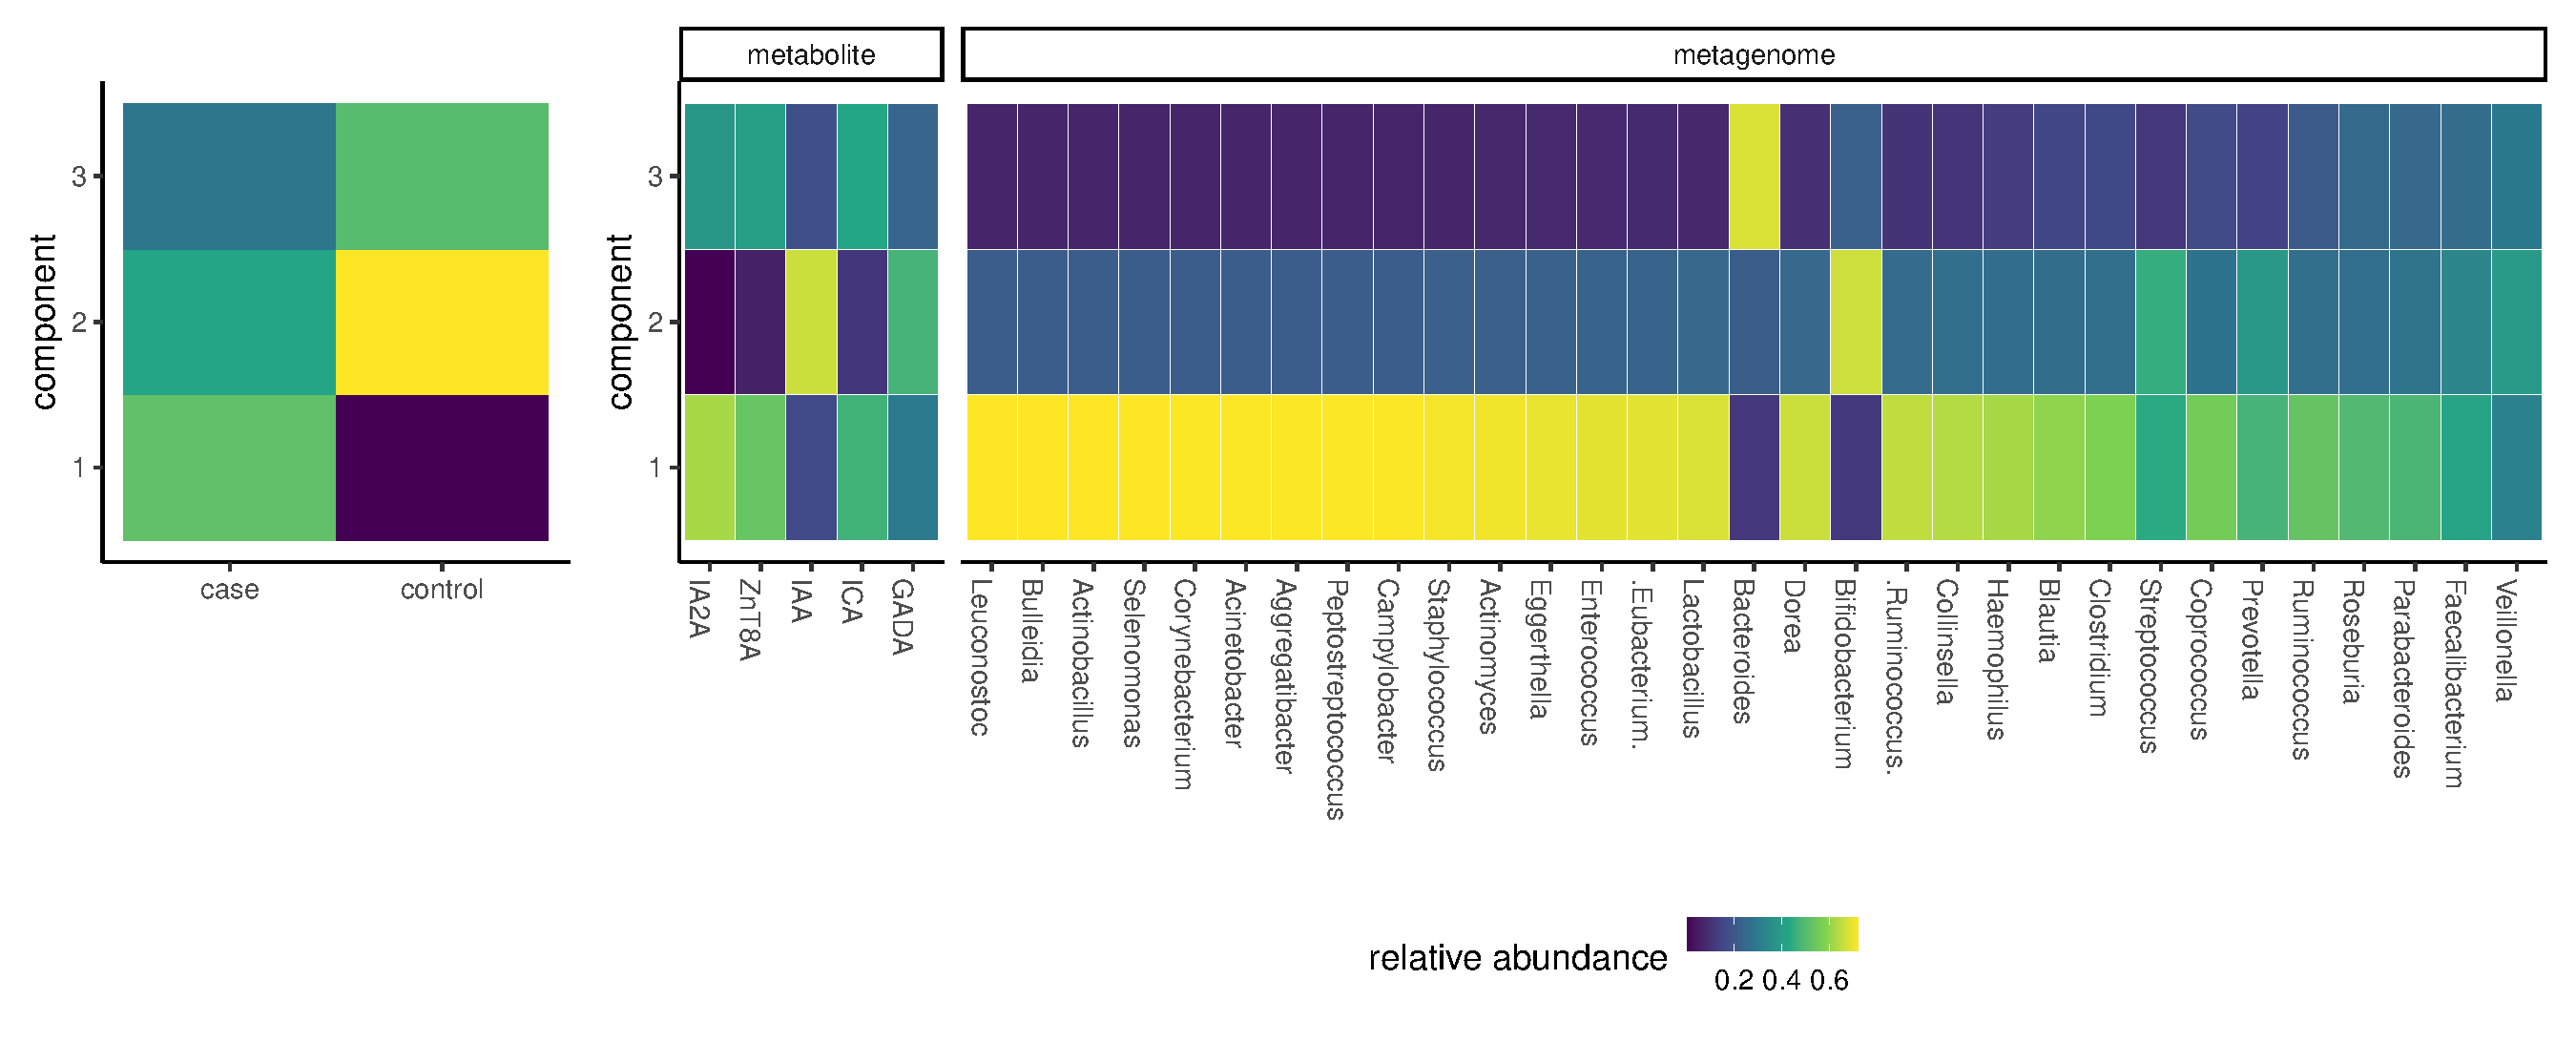
\includegraphics[width=0.9\textwidth]{img/Kostic_name.pdf}
\caption{推定された$V$の各 component に関連する細菌・代謝物. }
\end{figure}

component 1 が相対的に case (糖尿病) に多い. component 2, 3はそれぞれ \textit{Bifidobacterium}, \textit{Bacteroides} が特徴的. 
}


\begin{frame}
\frametitle{交互作用項について}

\begin{align*}
f_n =  \sum_{l}\prod_{d=1}^D v_{dl}^{x_{nd}} 
\end{align*}
と置く. $\circ$ をアダマール積(要素ごとの積)として,
\begin{block}{疑似コード}
\begin{itemize}
%\begin{flushleft}
\item[] $X$に交互作用なし:
$$
f[n] = \operatorname{sum}( v^{(1)}[\mathrm{cell}[n],:] \circ v^{(2)}[\mathrm{\color{RedOrange}{gene}}[n],:]  \circ  v^{(3)}[\mathrm{\color{RoyalBlue}{species}}[n],:] )
$$
\item[] $X$に{\color{RedOrange}{gene} } $\times$ {\color{RoyalBlue}{species} }の交互作用:
$$
f[n] = \operatorname{sum}(  v^{(1)}[{\mathrm{cell}}[n],:] \circ v^{(2)}[\mathrm{\color{RedOrange}{gene}}[n], \mathrm{\color{RoyalBlue}{species}}[n],:] )
$$
\end{itemize}
\end{block}

遺伝子と種の交互作用は遺伝子についての潜在変数に種ごとの変化を許す
\end{frame}

\begin{frame}
\frametitle{ヒトの遺伝子との既知の対応}

van Zyl \textit{et al.}(2020) データの分析では種をまたぐ共通因子として機能

\begin{figure}
\begin{tabular}{cc}
\begin{minipage}{0.5\textwidth}
\footnotesize
\begin{tabular}{cc}
mouse & human\\
\hline
Khdc1a, Khdc1b, Khdc1c& KHDC1, KHDC1L\\
Kcnq5& KCNQ5\\
Gm28237& - \\
\end{tabular}
\end{minipage}
&
\begin{minipage}{0.5\textwidth}
\centering
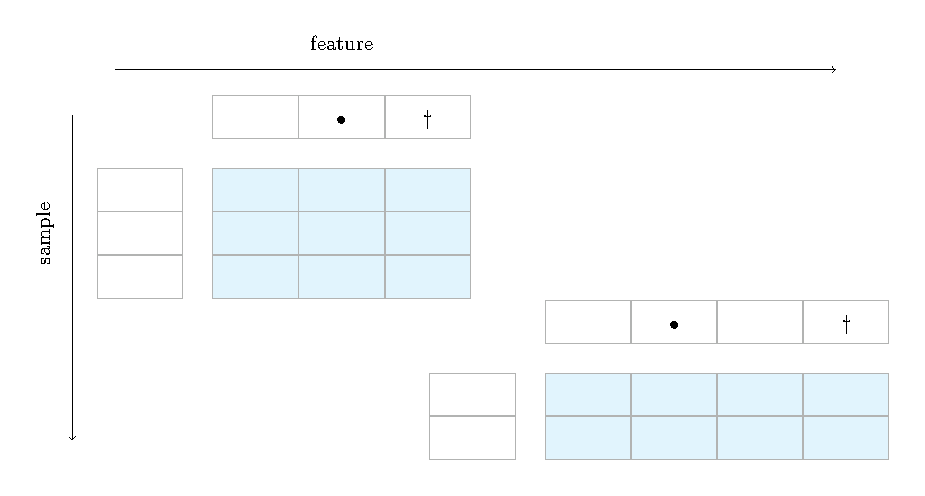
\includegraphics[width=0.8\textwidth]{img/anndata}  
\end{minipage}
\end{tabular}
\caption{マウスとヒトの遺伝子の既知の対応(一部を抜粋)}
\end{figure}
\end{frame}


\frame{
\frametitle{van Zyl \textit{et al.}(2020); 5種の哺乳類のRNA-seq }

\begin{figure}
\begin{tabular}{cc}
\subfloat[A2Mに近い]{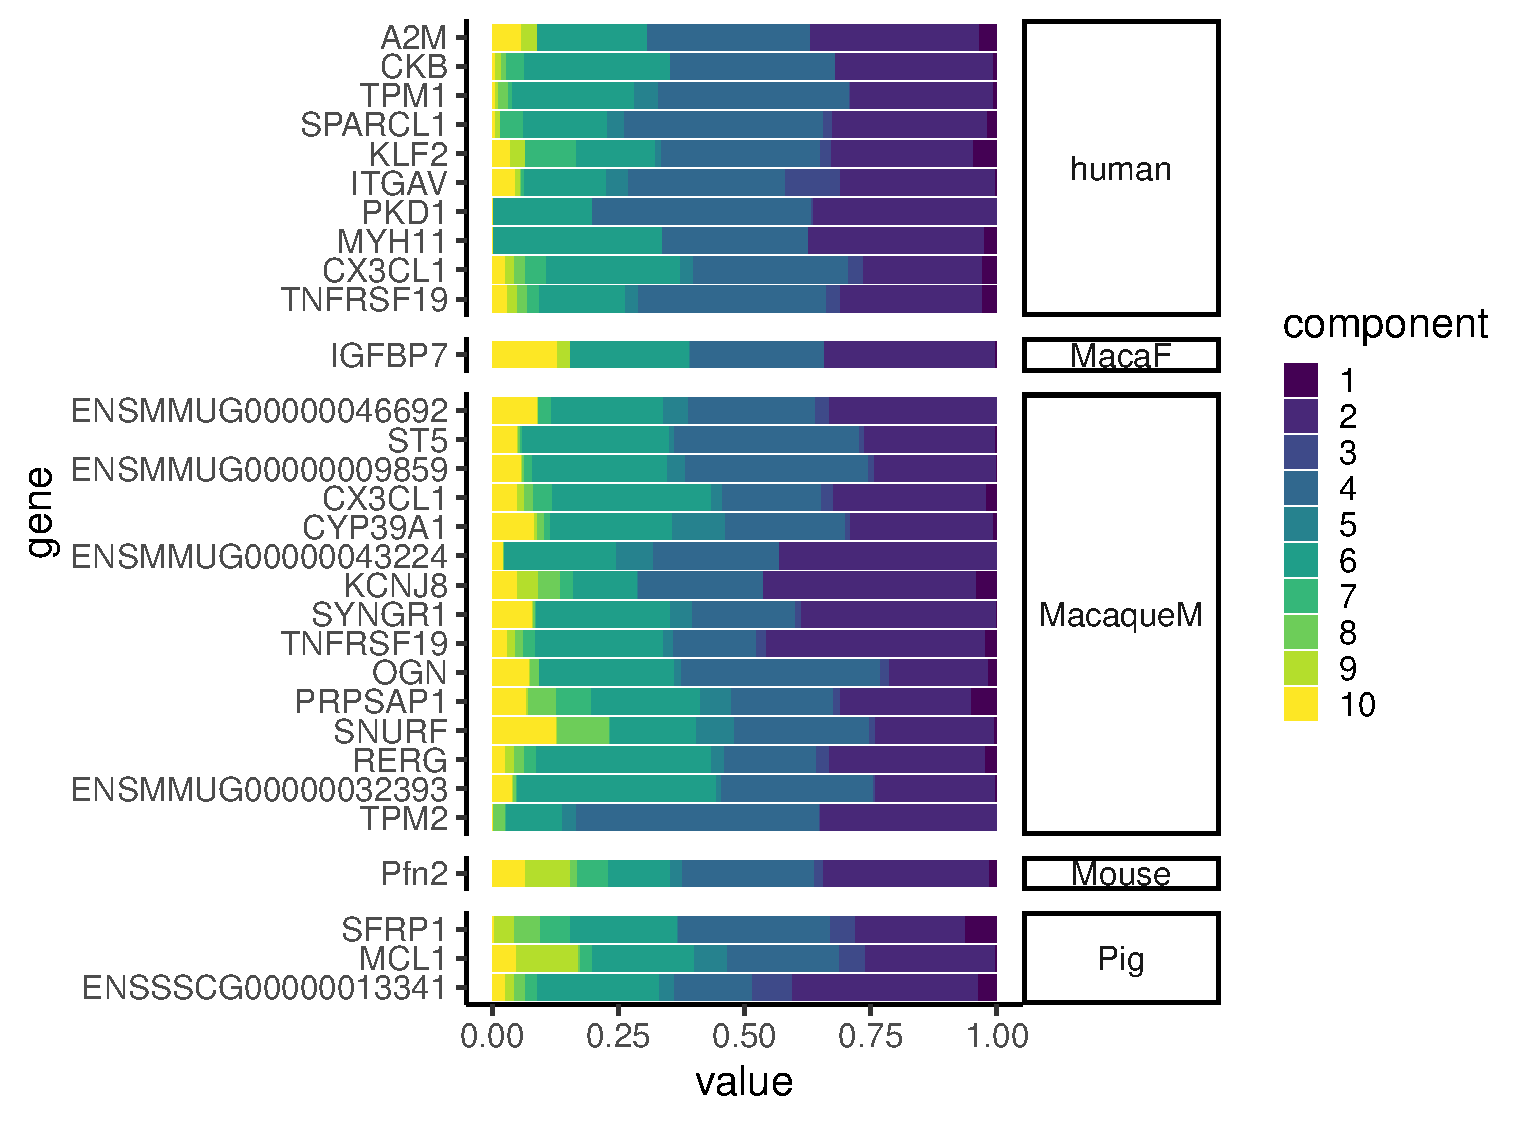
\includegraphics[width=0.48\textwidth]{img/a2m_similar10.pdf}} &
\subfloat[MYOCに近い]{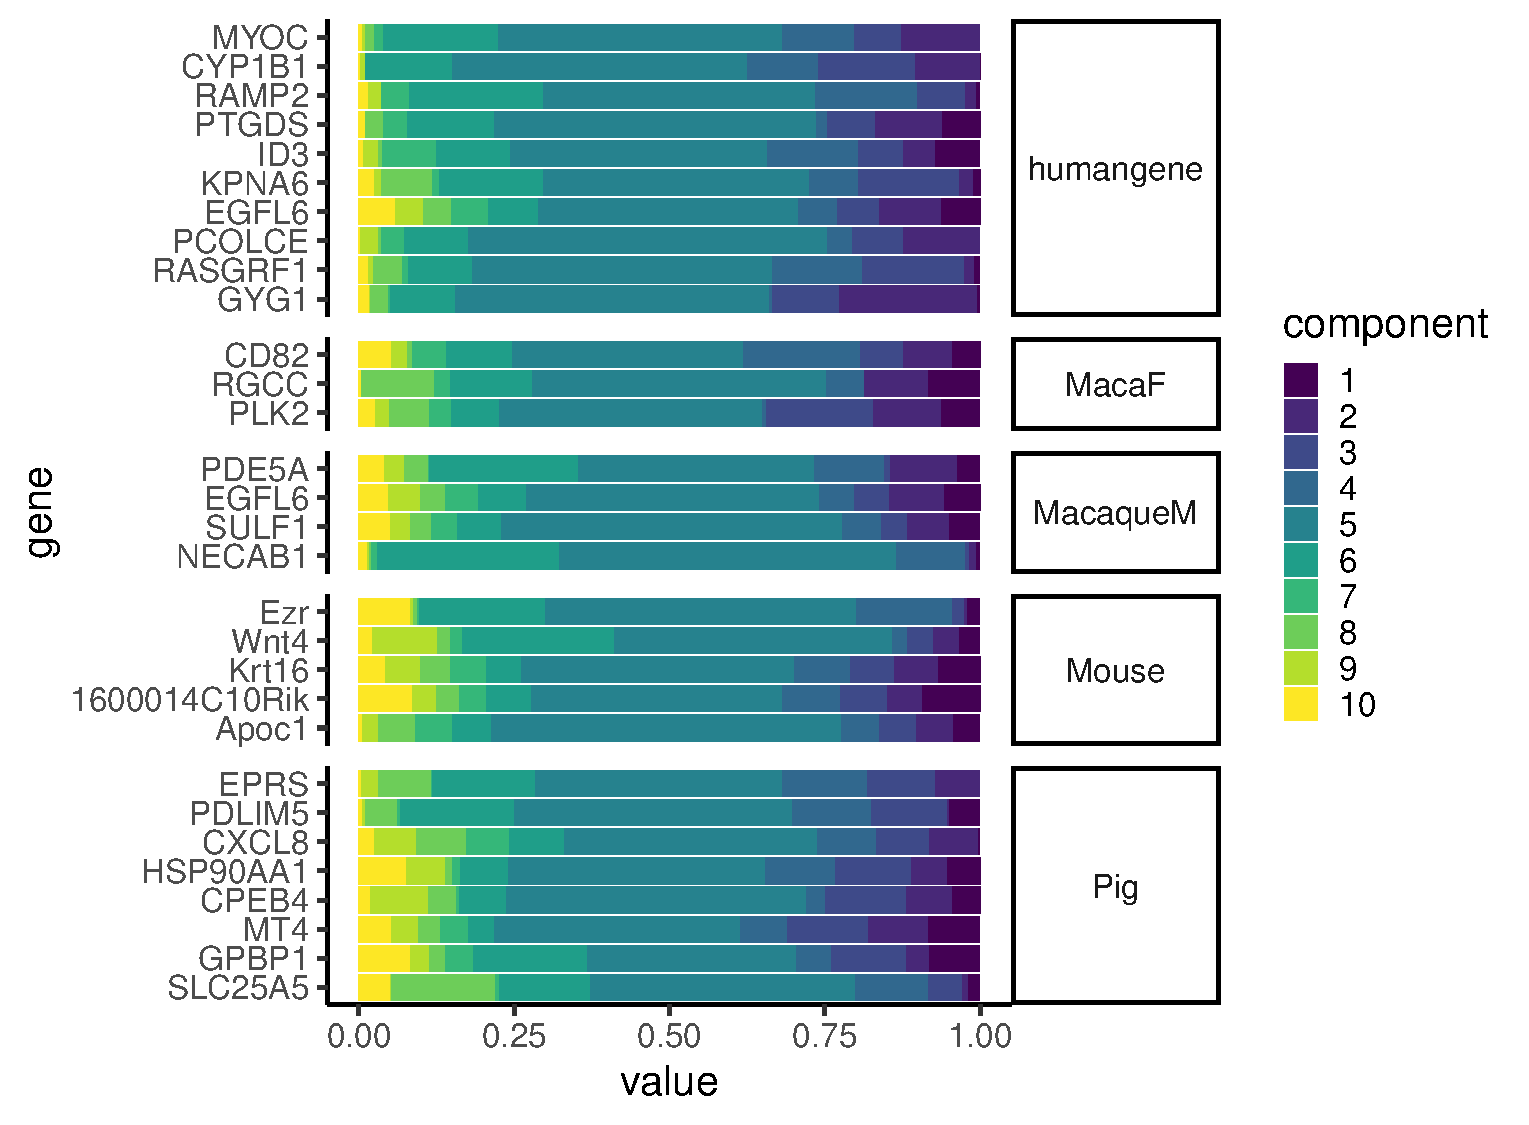
\includegraphics[width=0.48\textwidth]{img/myoc_similar10.pdf}}
\end{tabular}
\caption{推定された$V$を2乗距離で評価}
\end{figure}
}
\frame{
\frametitle{van Zyl \textit{et al.}(2020); A2M}
\begin{columns}
\begin{column}{0.5\textwidth}
\begin{figure}
\subfloat[A2Mに近い]{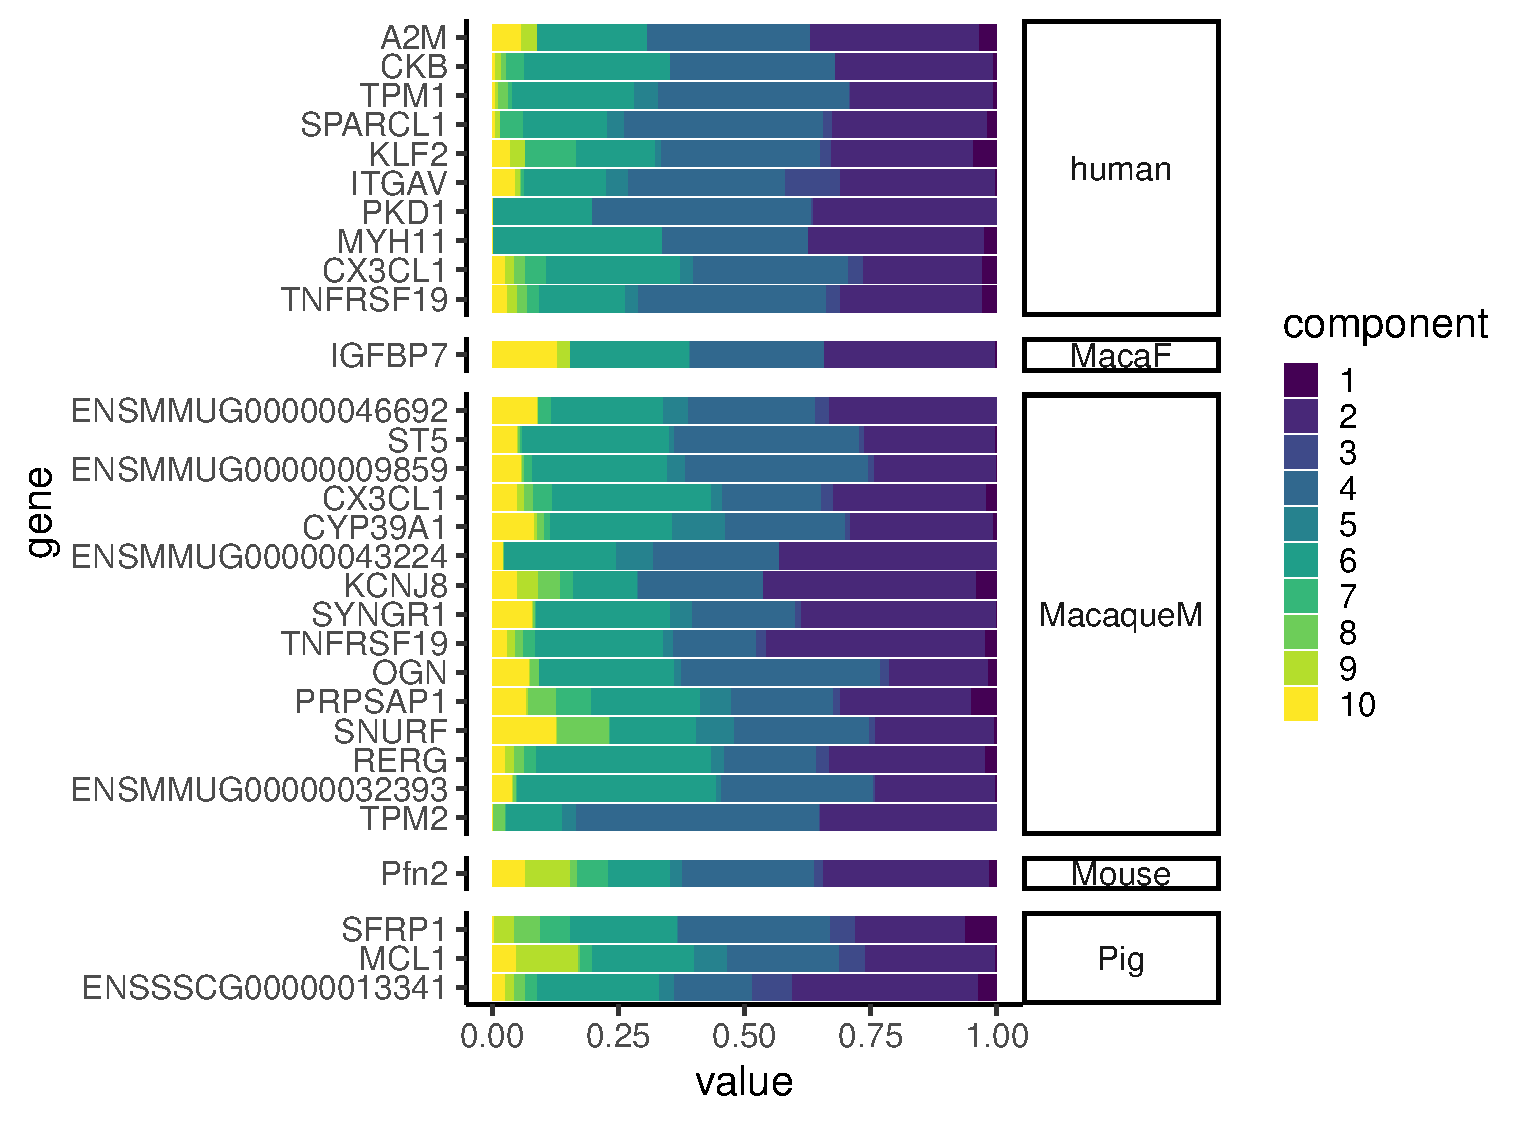
\includegraphics[width=\textwidth]{img/a2m_similar10.pdf}}
\end{figure}
\end{column}
\begin{column}{0.5\textwidth}
\footnotesize
\begin{itemize}
\item A2M: アルツハイマー病と関連 
\item CKB: 脳内および他の細胞内でホモ二量体として機能
\item TPM1: 横紋筋および平滑筋の収縮系および非筋肉細胞の細胞骨格に関与する
\item SPARCL1:解剖学的構造の発達とシナプス組織の調節に関与すると予測される
\item KLF2: 哺乳類の発生の初期に発現し多くの異なる細胞型で見られる
\end{itemize}
\footnotesize{National library of medicine. \url{https://www.ncbi.nlm.nih.gov/gene/} (最終アクセス日2024/5/20)}
\end{column}
\end{columns}
}
\frame{
\frametitle{van Zyl \textit{et al.}(2020); MYOC}
\begin{columns}
\begin{column}{0.5\textwidth}
\begin{figure}
\subfloat[MYOCに近い]{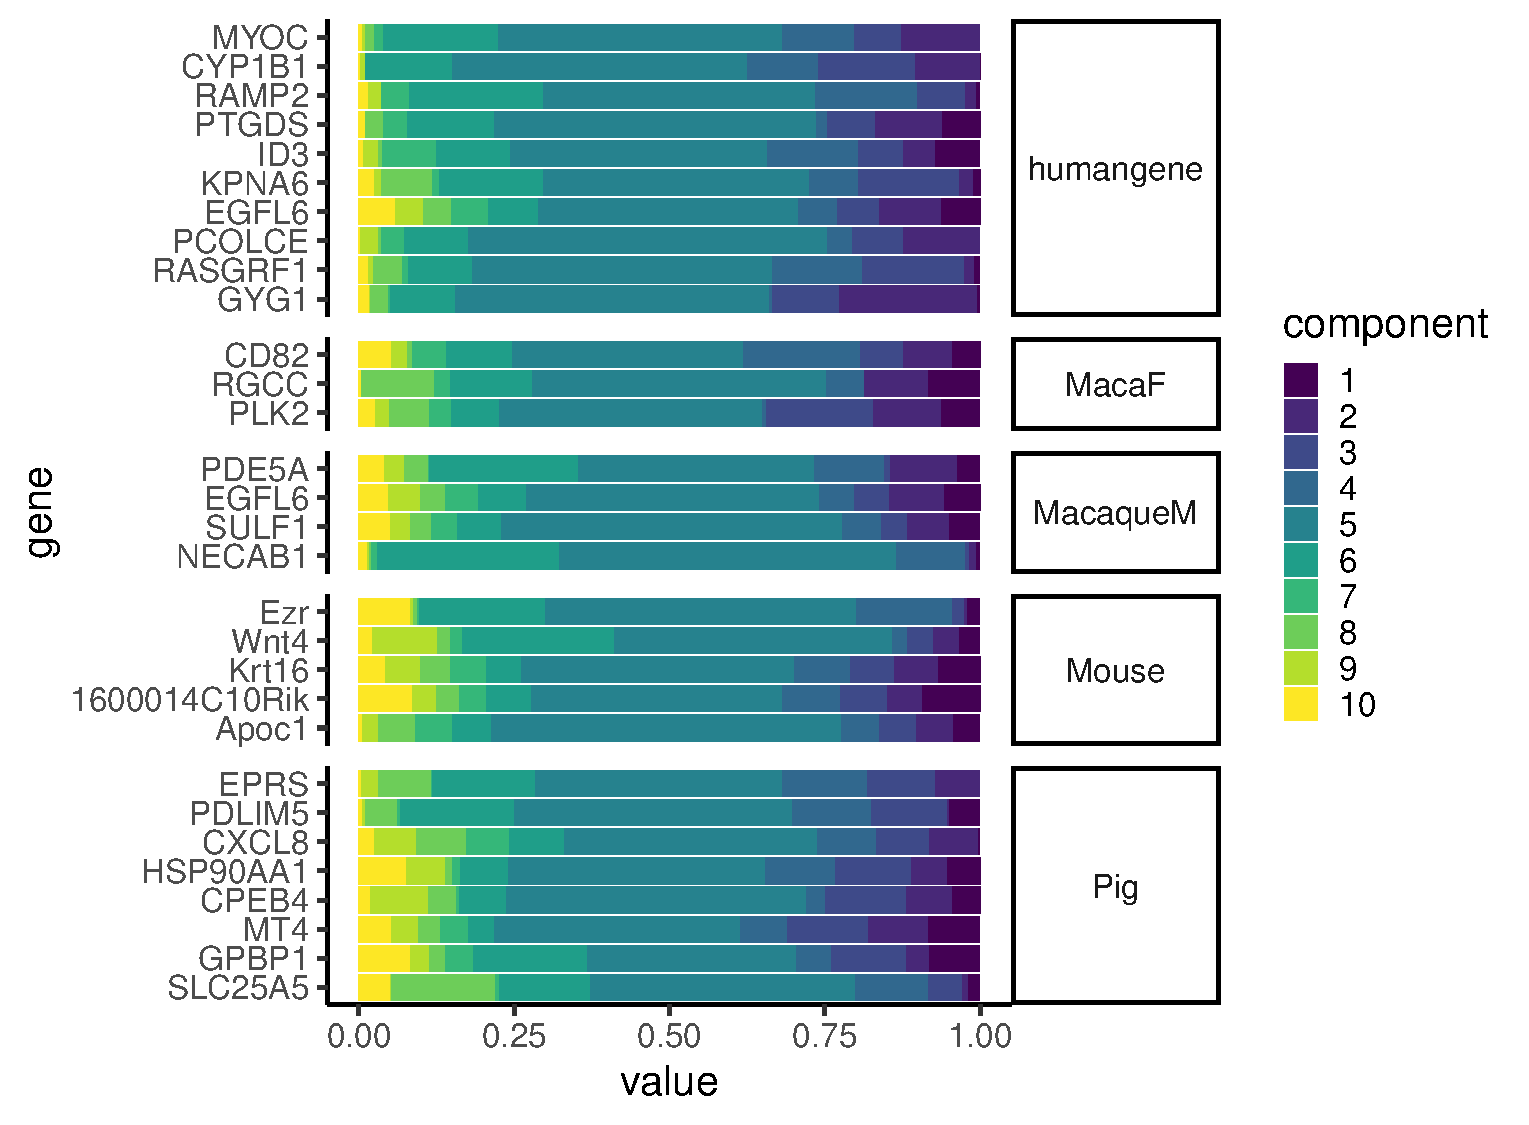
\includegraphics[width=\textwidth]{img/myoc_similar10.pdf}}
\end{figure}
\end{column}
\begin{column}{0.5\textwidth}
\footnotesize
\begin{itemize}
\item MYOC: 眼圧と関連
\item CYP1B1: この遺伝子の変異は原発性先天性緑内障と関連
\item RAMP2: グリコシル化とアドレノメデュリン受容体の細胞表面への輸送に関与
\item PTGDS: 平滑筋の収縮・弛緩に関与し, 脳で優先的に発現
\item ID3: この遺伝子によってコードされるタンパク質は他の HLH タンパク質とヘテロ二量体を形成
\end{itemize}
\footnotesize{National library of medicine. \url{https://www.ncbi.nlm.nih.gov/gene/} (最終アクセス日2024/5/20)}
\end{column}
\end{columns}
}
\frame{
\frametitle{まとめ}

テンソル分解(CP分解)を特殊な場合として含むモデルと, 変分ベイズ法に基づくその推定量を提案した.

\setbeamertemplate{itemize item}{\color{RedOrange}\checkmark}
\begin{itemize}
\item 多様なデータに適用できる柔軟性
\item 非負制約による解釈性
\end{itemize}

\structure{今後の発展:}大規模メタアナリシス, 因果推論, 時空間の相関を考慮
%(学習済みword2vec のようなイメージ)
%(g-formula)
}
\appendix
\begin{frame}[noframenumbering]
%\url{https://github.com/abikoushi/moltenNMF}
\end{frame}

\begin{frame}[noframenumbering]
\frametitle{例: 3階のテンソルの場合}
Data:
$$
 Y=(y_{ijk}), \quad y=(y_n) = \operatorname{vec}(Y) .
$$

CP分解:
\begin{equation*}
y_{ijk} \approx \sum_{l}v_{il}^{(1)} v_{jl}^{(2)} v_{kl}^{(3)}
\end{equation*}

UNMF\footnote{Ko ABE and Teppei SHIMAMURA (2023) UNMF: A unified non-negative matrix factorization for multi-dimensional omics data. Briefings in Bioinformatics. }:
\begin{equation*}
y_{n} \approx \sum_{l}\prod_{d=1}^D v_{dl}^{x_{nd}},  \quad x_{nd} \in \{0,1\}
\end{equation*}
ここで, 
\begin{align*}
V = (v_{dl}) = \left(V^{(1)} , V^{(2)} , V^{(3)}\right)'.
\end{align*}
\end{frame}

\begin{frame}[noframenumbering]
\frametitle{シミュレーション; 設定}

サンプル:
$$
y_{ij} \sim \mathrm{Poisson}\left(\sum_{l} w_{il}h_l{lj} \right), \quad  (i=1,\ldots,500, j=1,\ldots, 1000)
$$

行方向の傾向$W$と列方向の傾向$H$をそれぞれ基底関数($\sin(x)$, $\cos(x)$, $\mathrm{sign}(x)$, $\tanh(x)$)の一次結合で設定.

\begin{figure}
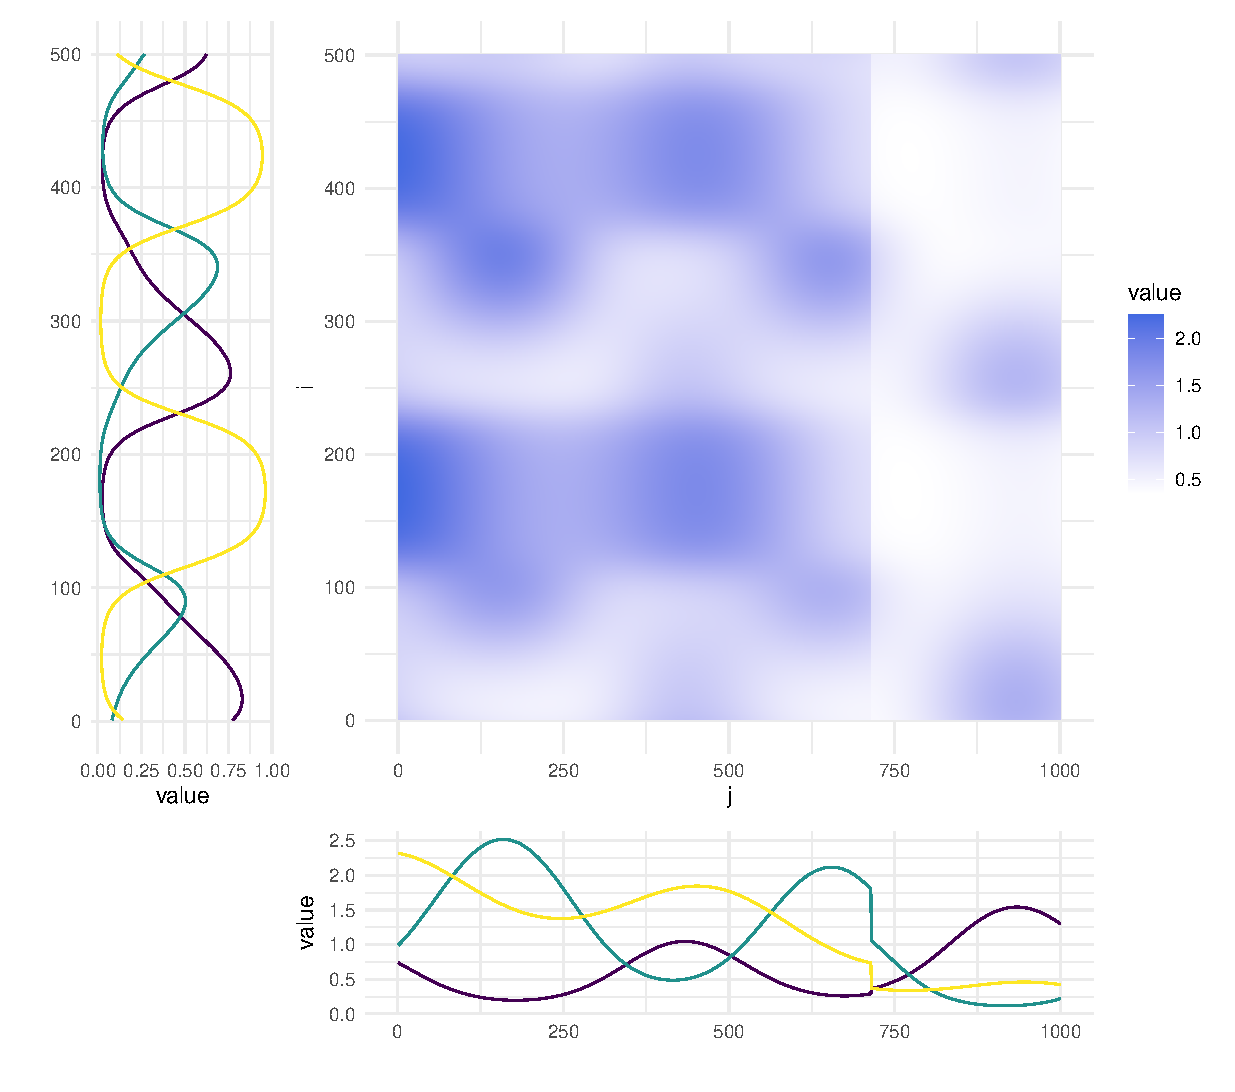
\includegraphics[width=0.4\textwidth]{img/groundtruth.pdf}
\caption{本シミュレーションで設定した真値}
\end{figure}
\end{frame}

\begin{frame}[noframenumbering]
\begin{figure}
\begin{tabular}{cc}
\subfloat[$L=3$]{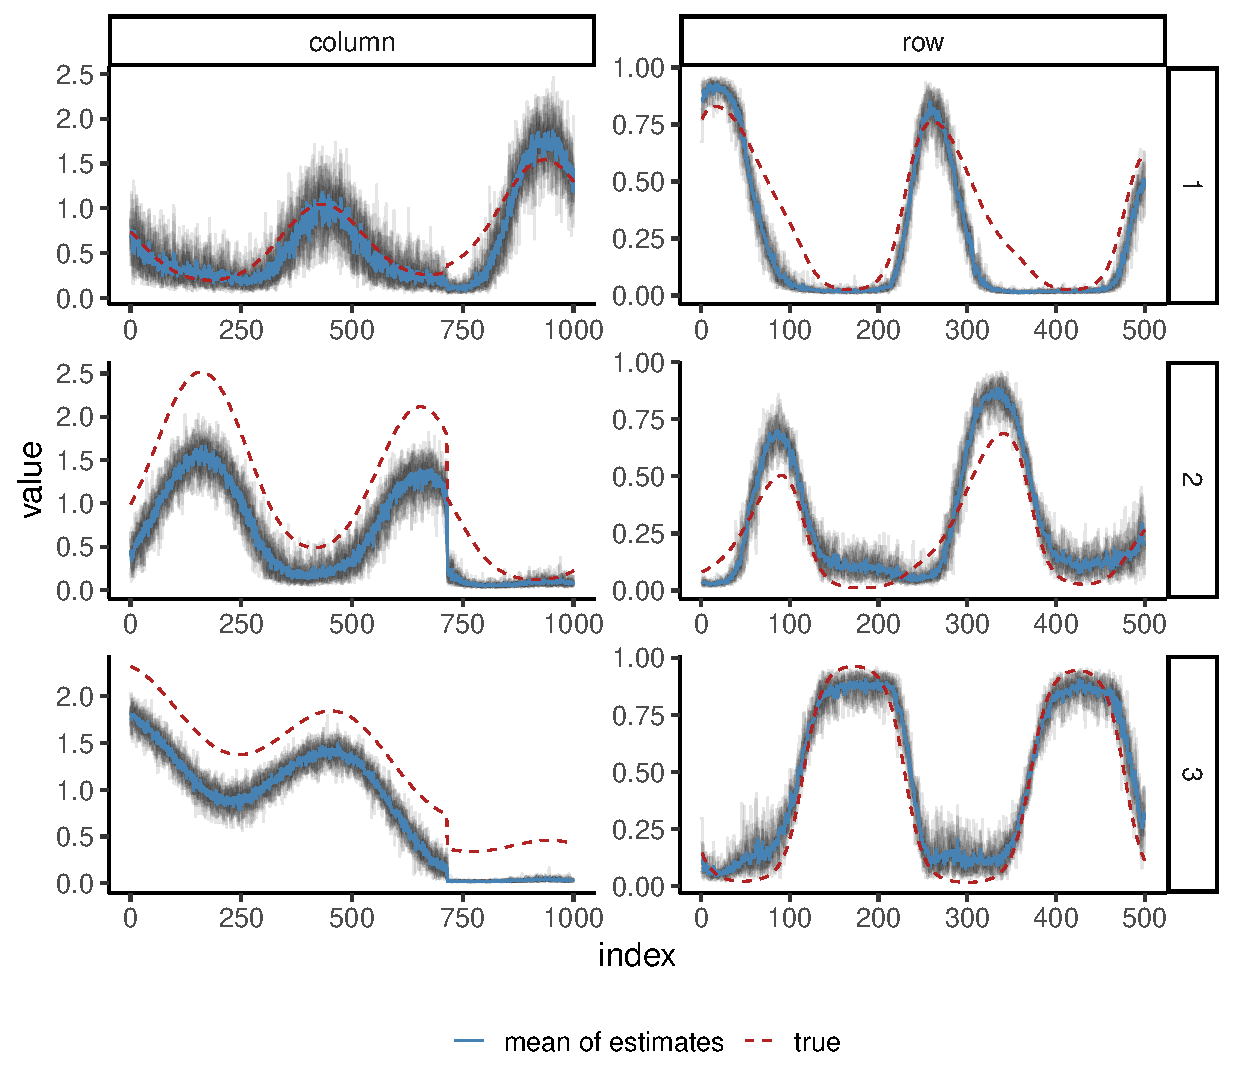
\includegraphics[width=0.48\textwidth]{img/multi_3to3.pdf}} &
\subfloat[$L=4$]{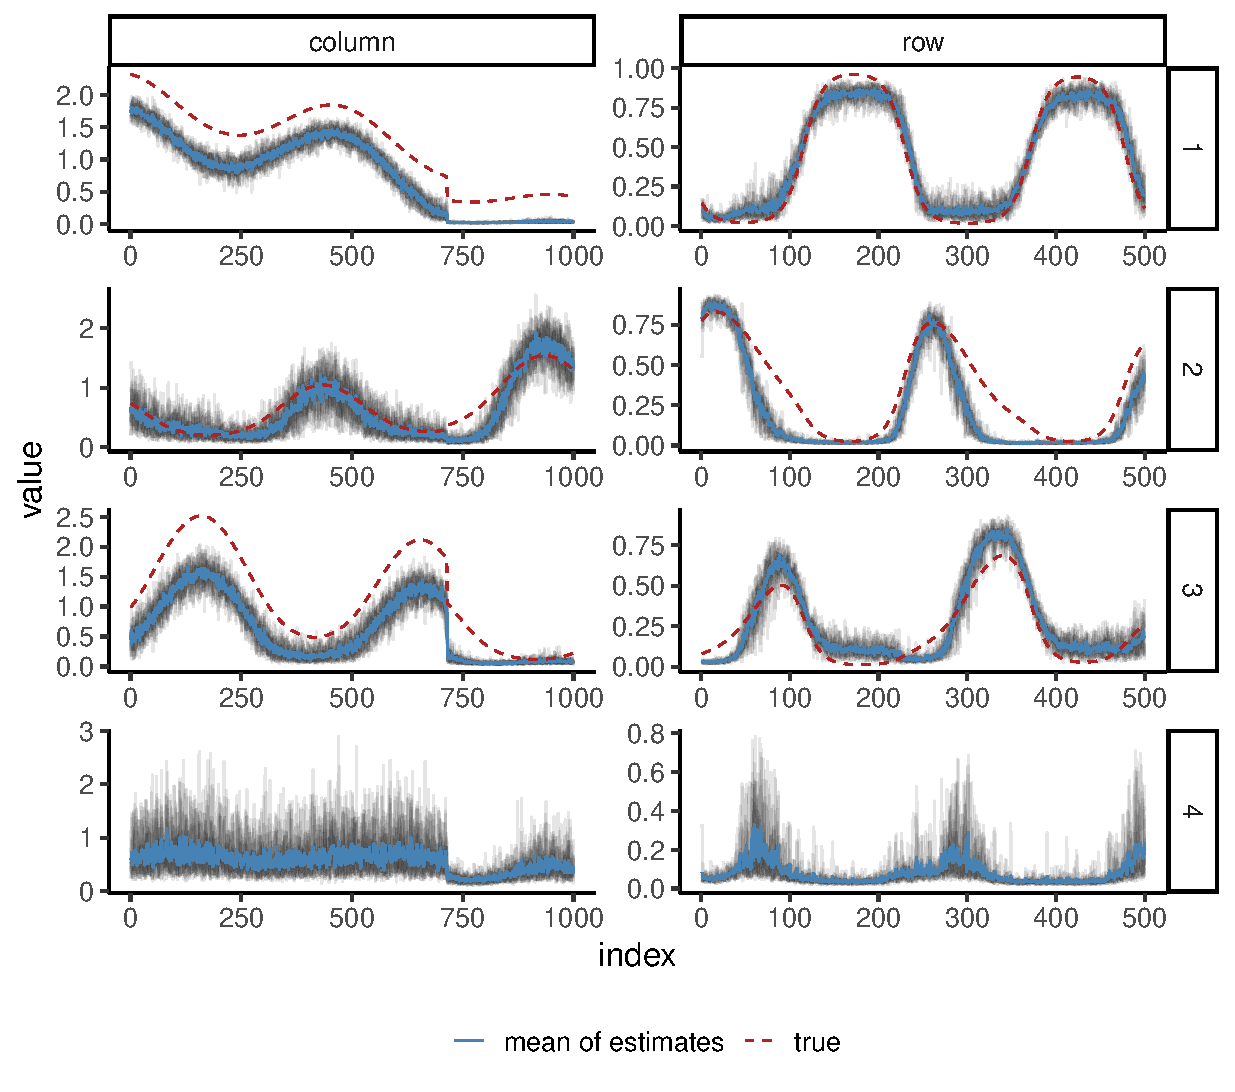
\includegraphics[width=0.48\textwidth]{img/multi_3to4.pdf}}
\end{tabular}
\end{figure}
\end{frame}

\begin{frame}[noframenumbering]
\url{https://github.com/abikoushi/moltenNMF}
\end{frame}
\end{document} 